\chapter{Existující algoritmy pro kompresi JSON}
\label{kapitolaJsonAlgoritmy}

JSON byl navržen jako odlehčená varianta způsobu formátování dat proti XML, čímž byla odstraněna i redundance při použití počátečního a ukončovacího tagu. Po seznámení s jeho definicí a syntaxí je zřejmé, že zde již nezbývá moc prostoru k dalšímu odlehčení. Podíváme-li se ale na data zapsaná v tomto formátu, která mohou obsahovat například výstup SQL příkazu SELECT nad databází (viz \textcolor{red}{odkaz na testovací soubor}), můžeme vidět, že se zde některé prvky přece jen opakují. Jsou to klíče, včetně uvozovek, v jednotlivých objektech, které stačí zapsat pouze jednou. Tohoto poznatku využívají i dva vybrané algoritmy JSONH a CJSON, které jsou specifické tím, že výstupem z nich je validní JSON. Rád bych čtenáře upozornil, že algoritmů pro kompresi JSON neexistuje mnoho, resp. jsou si velice podobné myšlenkou, provedením i názvy.

S daty v tomto formátu nepracujeme jako s obyčejným textem, ale převedeme do paměti jako hodnoty (pole, objekty atd.), což odpovídá zpracování pomocí JavaScriptu. Tomu odpovídá i terminologie použitá v této kapitole, která byla popsána v části \ref{syntaxeJson}.

\section{JSONH}
\label{jsonh}
Tento algoritmus dovoluje komprimovat pouze homogenní kolekce dat, v terminologii JSON jde o pole objektů, které mají stejný počet klíčů se stejnými názvy. Homogenitu dat musí zaručit uživatel, algoritmus samotný toto nikterak neošetřuje. Autor projektu JSONH \cite{jsonh}, kde je algoritmus implementován, na serveru github.com uvádí, že data mohou být v některých případech zmenšena až na 30 \%.

\subsection{Vzorová data}
Mějme homogenní kolekci zaměstnanců firmy, ve které máme uložené databázové id, příjmení a pozici, na které zaměstnanec pracuje. Část této kolekce vypadá následujícím způsobem:

\texttt{[\{ \textquotedblright id\textquotedblright : 1, \textquotedblright name\textquotedblright : \textquotedblright Sánchez\textquotedblright, \textquotedblright position\textquotedblright : \textquotedblright Manager\textquotedblright\ \},\\
\hspace*{2.3mm}\{ \textquotedblright id\textquotedblright : 2, \textquotedblright name\textquotedblright : \textquotedblright Duffy\textquotedblright, \textquotedblright position\textquotedblright : \textquotedblright Programmer\textquotedblright\ \},\\
\hspace*{2.3mm}\{ \textquotedblright id\textquotedblright : 3, \textquotedblright name\textquotedblright : \textquotedblright Tamburello\textquotedblright, \textquotedblright position\textquotedblright : \textquotedblright Worker\textquotedblright\ \}]}

\subsection{Postup komprese}
\begin{enumerate}
\item Textová data jsou převedena na pole objektů.
\item \label{jsonhItem0} Z prvního objektu v poli jsou určeny klíče a jejich počet.
\item \label{jsonhItem1} Ze všech objektů v poli jsou postupně vyzvednuty hodnoty pro příslušné klíče, přičemž je zachováno pořadí klíčů, jak jsme jej získali v kroku \ref{jsonhItem0}.
\item Je vytvořeno pole, které obsahuje prvky: počet klíčů, seznam klíčů a hodnoty vyzvednuté v kroku \ref{jsonhItem1}.
\item Vytvořené pole serializujeme jako JSON do řetězce nebo souboru.
\end{enumerate}

Data po kompresi mají následující podobu:

\texttt{[ 3, \textquotedblright id\textquotedblright, \textquotedblright name\textquotedblright, \textquotedblright position\textquotedblright, 1, \textquotedblright Sánchez\textquotedblright, \textquotedblright Manager\textquotedblright, 2, \textquotedblright Duffy\textquotedblright,\\
\hspace*{5mm}\textquotedblright Programmer\textquotedblright, 3, \textquotedblright Tamburello\textquotedblright, \textquotedblright Worker\textquotedblright\ ]}

\subsection{Postup rekonstrukce dat}
\begin{enumerate}
\item Textová data jsou převedena na pole hodnot.
\item Z prvního prvku v poli určíme počet klíčů, označíme $n$.
\item Z prvků 2 až $n+1$ určíme klíče.
\item Z následujících prvků (po $n+1$) rekonstruujeme původní objekty až do konce pole a ukládáme je do pole nového.
\item Nové pole serializujeme jako JSON do řetězce nebo souboru.
\end{enumerate}

\section{CJSON}
\label{cjson}
Proti JSONH dokáže algoritmus CJSON komprimovat i nehomogenní data. K tomu, aby bylo při kompresi dosaženo významné úspory, je nutná určitá struktura dat. Tu bych přirovnal k dědičnosti, jak ji známe z principů objektově orientovaného programování. To znamená, že data lze popsat pomocí tříd, které sdílejí některé členy. Účinnost komprese závisí na poměru počtu tříd a množství dat k nim příslušných. Platí, že čím menší počet tříd a větší množství příslušných dat, tím větší je kompresní účinnost. Za ideál lze potom považovat homogenní data, tedy případ kdy stačí k popisu pouze jedna třída, ke které přísluší všechna data.

Algoritmus v průběhu komprese vytváří postupně strom šablon, který je na závěr vložen do výstupu ve formě jednotlivých šablon, která využívá již zmiňované dědičnosti. Konstrukce stromu je zobrazena na obrázku \ref{cjsonKonstrukceStromu}. \textcolor{red}{Doplnit očíslování v obrázku a popis vytváření stromu.}

\begin{figure}[!htb]
\centering
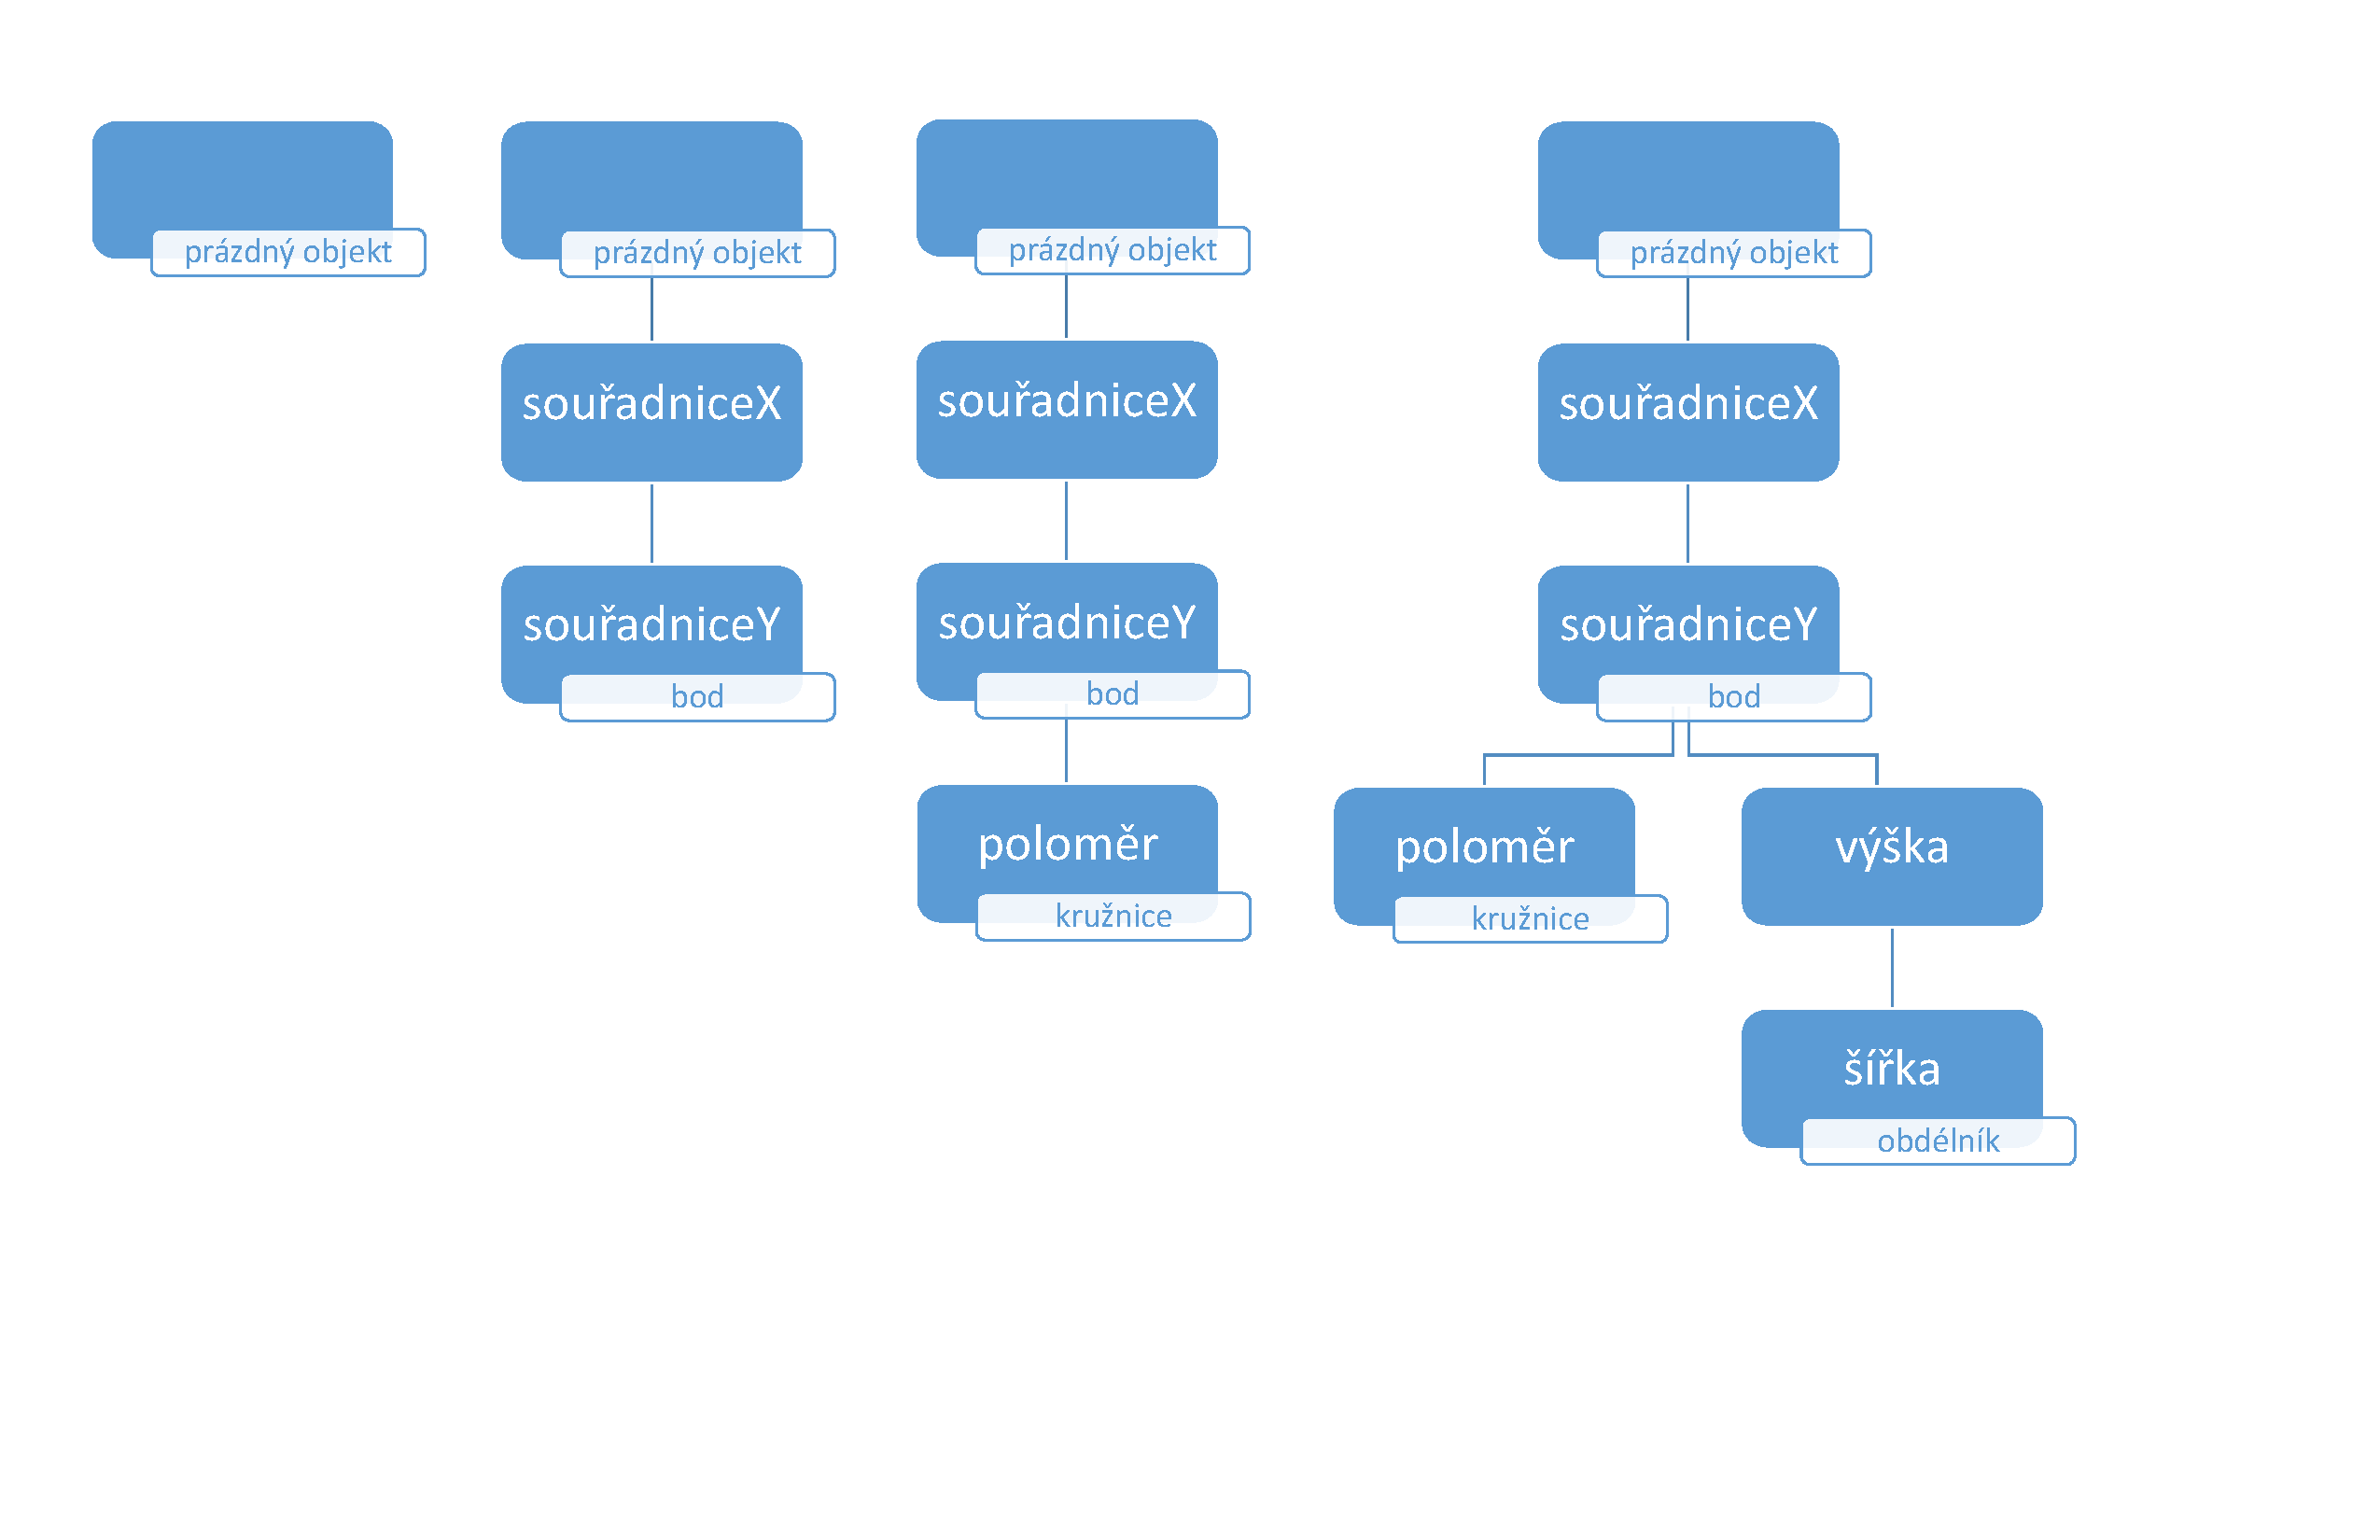
\includegraphics[trim=30 180 150 50, clip, angle=0, width=150mm]{cjsonStrom}
\caption{Postup vytvoření stromu šablon}
\label{cjsonKonstrukceStromu}
\end{figure}

\subsection{Vzorová data}
\textcolor{red}{Vytvořit data, popsat, upravit obrázek konstrukce stromu!!!}

Mějme homogenní kolekci zaměstnanců firmy, ve které máme uložené databázové id, příjmení a pozici, na které zaměstnanec pracuje. Tato kolekce může vypadat následujícím způsobem.

\texttt{[\\
\hspace*{5mm}\{ \textquotedblright id\textquotedblright : 1, \textquotedblright name\textquotedblright : \textquotedblright Sánchez\textquotedblright, \textquotedblright position\textquotedblright : \textquotedblright Manager\textquotedblright\ \},\\
\hspace*{5mm}\{ \textquotedblright id\textquotedblright : 2, \textquotedblright name\textquotedblright : \textquotedblright Duffy\textquotedblright, \textquotedblright position\textquotedblright : \textquotedblright Programmer\textquotedblright\ \},\\
\hspace*{5mm}\{ \textquotedblright id\textquotedblright : 3, \textquotedblright name\textquotedblright : \textquotedblright Tamburello\textquotedblright, \textquotedblright position\textquotedblright : \textquotedblright Worker\textquotedblright\ \}\\
]}

\subsection{Postup komprese}
\label{cjsonPoKompresi}
\begin{enumerate}
\item Textová data jsou převedena na pole objektů.
\item Ze všech objektů v poli jsou postupně vyzvednuty hodnoty a uloženy do nového pole objektů. Tyto objekty obsahují pouze pole příslušných hodnot. Zároveň je konstruován strom šablon.
\item Ze stromu šablon je vytvořeno pole šablon. Šablona je pole obsahující identifikátor šablony, ze které dědí, a klíče. Identifikátor 0 je rezervován pro šablonu odpovídající prázdnému objektu.
\item Objekty s hodnotami jsou doplněny o identifikátor odpovídající šablony.
\item \label{cjsonItem0}Ze vzniklých polí vytvoříme objekt obsahující identifikátor kompresního algoritmu (klíč \texttt{"f"}), pole šablon (klíč \texttt{"t"}) a pole hodnot (klíč \texttt{"v"}) (viz \ref{cjsonPoKompresi}).
\item Objekt vzniklý v bodu \ref{cjsonItem0} serializujeme jako JSON do řetězce nebo souboru.
\end{enumerate}

Data mají po kompresi následující tvar:

\texttt{\{\hspace*{3mm}"f" : "cjson",\\
\hspace*{5mm}"t" : [ [ 0, "x", "y" ], [ 1, "width", "height" ] ],\\
\hspace*{5mm}"v" : [ \{ "" : [ 1, 100, 100 ] \}, \{ "" : [ 2, 100, 100, 200, 150 ] \} ] \}}

\subsection{Postup rekonstrukce dat}
\begin{enumerate}
\item Textová data jsou převedena na pole hodnot.
\item Vytvoříme pole, do kterého postupně vkládáme objekty vzniklé z prvků pole hodnot a příslušných šablon.
\item Tuto kolekci serializujeme jako JSON do řetězce nebo souboru.
\end{enumerate}